\documentclass[xcolor=x11names,compress]{beamer}

%% General document %%%%%%%%%%%%%%%%%%%%%%%%%%%%%%%%%%
\usepackage{graphicx}
\usepackage{tikz}
\usetikzlibrary{decorations.fractals,lindenmayersystems}
%%%%%%%%%%%%%%%%%%%%%%%%%%%%%%%%%%%%%%%%%%%%%%%%%%%%%%


%% Beamer Layout %%%%%%%%%%%%%%%%%%%%%%%%%%%%%%%%%%
\useoutertheme[subsection=false,shadow]{miniframes}
\useinnertheme{default}
\usefonttheme{serif}
\usepackage{palatino}

\setbeamerfont{title like}{shape=\scshape}
\setbeamerfont{frametitle}{shape=\scshape}

\setbeamercolor*{lower separation line head}{bg=DeepSkyBlue4} 
\setbeamercolor*{normal text}{fg=black,bg=white} 
\setbeamercolor*{alerted text}{fg=red} 
\setbeamercolor*{example text}{fg=black} 
\setbeamercolor*{structure}{fg=black} 
 
\setbeamercolor*{palette tertiary}{fg=black,bg=black!10} 
\setbeamercolor*{palette quaternary}{fg=black,bg=black!10} 

\setbeamertemplate{blocks}[rounded][shadow=true]
\setbeamercolor{block title}{bg=black!50!white}
\setbeamercolor{block title example}{bg=black!50!white}
\setbeamercolor{block body}{bg=black!15!white}
\setbeamercolor{block body example}{bg=black!15!white}

\setbeamertemplate{navigation symbols}{}
%%%%%%%%%%%%%%%%%%%%%%%%%%%%%%%%%%%%%%%%%%%%%%%%%%

\author[Francisco Blanco-Silva]{Francisco Blanco-Silva}
\institute[USC]{University of South Carolina}
\date{
    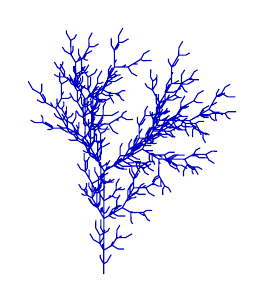
\begin{tikzpicture} 
    \draw [blue!75!black, rotate=90]
    [l-system={rule set={F -> FF-[-F+F]+[+F-F]}, axiom=F, order=4, step=2pt, 
        randomize step percent=25, angle=30, randomize angle percent=5}]
    lindenmayer system; 
    \end{tikzpicture}
    \\
    \today
}
\title{Lesson 5: Separable Equations. Singular Solutions}

\begin{document}

\frame{\titlepage}

\section{What do we know?}
\begin{frame}\frametitle{What do we know?}
\begin{itemize}[<+-|alert@+>]
\item The concept of a differential equation 
\begin{equation*}
F\big(x,y,y',\dotsc,y^{(n)}\big)=0
\end{equation*}
\item The concept of \textbf{order} of a differential equation.
\item The concept of a \textbf{general solution}
\item The concepts of an \textbf{initial value problem} (IVP) and \textbf{particular solution}.
\item Slope fields
\item Approximations to solutions via \textbf{Euler's Method} and \textbf{Improved Euler's Method}
\end{itemize} 
\end{frame}

\section{Separable Equations}
\subsection{Definition}
\begin{frame}\frametitle{Separable Equations}
\framesubtitle{Definition}
The first order equation $y'=H(x,y)$ is called \alert{separable} if we can write $H(x,y)$ as the product of a function of $x$ and a function of $y$: 
\begin{equation*}
H(x,y)=H_1(x)H_2(y)
\end{equation*}
\pause
We may find general solutions by simple integration:
\begin{align*}
 \uncover<3->{\frac{dy}{dx} &=H_1(x)H_2(y) \\}
 \uncover<4->{\frac{dy}{H_2(y)} &=H_1(x)\, dx \\}
 \uncover<5->{\int \frac{dy}{H_2(y)} &= \int H_1(x)\, dx}
\end{align*}

\pause\pause\pause\pause Solutions found this way may be expressed \alert{explicitly} (that is, solving for $y$ after integration), or \alert{implicitly} (without solving for $y$)
\end{frame}

\subsection{Examples}
\begin{frame}\frametitle{Separable Equations}
   \framesubtitle{Examples} 
   \begin{example}
        Find a particular solution of the initial value problem
        \begin{align*}
            y'&=6x(y-1)^{2/3} &y(0)&=7 
         \end{align*} 
   \end{example}
   \pause
   We start by re-arranging the equation and taking integrals:
   \begin{align*}
      \uncover<2->{\frac{dy}{dx}&= \overbrace{6x}^{H_1(x)} \overbrace{(y-1)^{2/3}}^{H_2(y)} &\int \frac{dy}{(y-1)^{2/3}} &= \int 6x\, dx \\}
      \uncover<3->{\alert<3>{3(y-1)^{1/3}} &\alert<3>{= 3x^2 + C}}
   \end{align*}
   \pause\pause To solve the IVP, we need to force $y(0)=7$:
   \begin{align*}
      \uncover<5->{3(7-1)^{1/3} &= 3 \cdot 0^2 + C &C &= 3\cdot 6^{1/3} \\}
      \uncover<6->{\alert{\text{Solution: } (y-1)^{1/3}} &\alert{= x^2 + 6^{1/3}}    }
   \end{align*}
\end{frame}

\begin{frame}\frametitle{Separable Equations}
\framesubtitle{Examples}
   \begin{example}
        Find a particular solution of the initial value problem
        \begin{align*}
            y'&=6x(y-1)^{2/3} &y(0)&=7 
         \end{align*} 
   \end{example}
   Note the form of the solution:
   \begin{equation*}
       (y-1)^{1/3}=x^2 + 6^{1/3} 
    \end{equation*} 
    This is \alert{implicit}.  If we want to provide an \alert{explicit} solution, we need to solve for $y$:
    \begin{align*}
       \uncover<2->{y-1 &= \big( x^2 + 6^{1/3} \big)^3 \\}
       \uncover<3->{y &= 1 + \big( x^2 + 6^{1/3} \big)^3}
    \end{align*}
\end{frame}

\begin{frame}\frametitle{Separable Equations}
\framesubtitle{Examples}
\begin{examples}
   Find a general solution (implicit) of the equation
   \begin{equation*}
      y' = \frac{(x-1)y^5}{x^2(2y^3-y)} 
   \end{equation*}
\end{examples}
\begin{align*}
   \uncover<2->{\frac{dy}{dx} &= \frac{x-1}{x^2} \cdot \frac{y^5}{y(2y^2-1)}\\} 
   \uncover<3->{\frac{2y^2-1}{y^4}\, dy &= \big( x^{-1} - x^{-2} \big)\, dx \\}
   \uncover<4->{\int \big( 2y^{-2} - y^{-4} \big)\, dy &= \int \big( x^{-1} - x^{-2} \big)\, dx \\}
   \uncover<5->{\alert{-2y^{-1} + \tfrac{1}{3} y^{-3}} &\alert{= \ln \lvert x \rvert + x^{-1} + C}}
\end{align*}
\end{frame}

\begin{frame}\frametitle{Separable Equations}
\framesubtitle{Examples}
Sometimes, equations that \emph{don't look separable} may be so, if manipulated accordingly.
\begin{example}
    Find a general solution (implicit) of the equation
    \begin{equation*}
        y'=1+x+y+xy 
     \end{equation*} 
 \end{example} 
 \pause  This does not look separable at first sight, but by factoring the $y$ and collecting like-terms, we obtain a more pleasant expression:
 \begin{columns}[T]
 \begin{column}{0.4\linewidth}
 \begin{align*}
    \uncover<3->{y' &= 1+x+\alert<3>{y}+x\alert<3>{y} \\}
    \uncover<4->{y' &= \alert<4>{1+x}+y\alert<4>{(1+x)} \\}
    \uncover<5->{y' &= (1+y)(1+x) \\}
 \end{align*}
 \end{column}
 \begin{column}{0.4\linewidth}
 \begin{align*}
    \uncover<6->{\frac{dy}{1+y} &= (1+x)\, dx \\}
    \uncover<7->{\int \frac{dy}{1+y} &= \int (1+x)\, dx \\}
    \uncover<8->{\alert{\ln \lvert 1+y\rvert} &\alert{= x+\tfrac{1}{2}x^2 + C}}
 \end{align*}
 \end{column}
 \end{columns}
\end{frame}

\begin{frame}\frametitle{Separable Equations}
\framesubtitle{Examples}
\begin{example}
  Find a general solution (implicit) of the differential equation
  \begin{equation*}
       \tan x\, \frac{dy}{dx} = y 
    \end{equation*}  
\end{example}
\begin{columns}[T]
    \begin{column}{0.45\linewidth}
        \begin{align*}
           \uncover<2->{\frac{dy}{y} &= \cot x dx \\}
           \uncover<3->{\int \frac{dy}{y} &= \int \frac{\cos x}{\sin x}\, dx}
       \end{align*}
    \end{column}
    \begin{column}{0.45\linewidth}
       \begin{align*}
           \uncover<4->{\ln \lvert y \rvert &= \ln \lvert \sin x \rvert + C\\}
           \uncover<5->{e^{\ln \lvert y \rvert} &= e^{\ln \lvert \sin x \rvert}\, \underbrace{e^C}_{A} \\}
           \uncover<6->{\alert{\lvert y \rvert} &\alert{= A \lvert \sin x \rvert }}
        \end{align*}
    \end{column}
\end{columns}

\end{frame}

\section{Singular Solutions}
\subsection{Motivation and Definition}
\begin{frame}[awhat]\frametitle{Singular Solutions}
\framesubtitle{Motivation and Definition}
Let us examine the previous equations again, with their found general solutions:
\begin{align*}
   y' &= 6x\alert{(y-1)}^{2/3} & (y-1)^{1/3} &=x^2+C \only<2>{&\alert{y}&\alert{=1}}\\
   y' &= \frac{x-1}{x^2} \cdot \frac{\alert{y^5}}{2y^3-y} &\tfrac{1}{3}y^{-3} -2y^{-1} &=\ln\lvert x\rvert + \tfrac{1}{x} + C \only<2>{&\alert{y}&\alert{=0}}\\
   y' &= (1+x)\alert{(1+y)} &\ln \lvert 1+y \rvert &= x+ \tfrac{1}{2}x^2 + C \only<2>{&\alert{y}&\alert{=-1}} \\
   \tan &x \frac{dy}{dx} = \alert{y} & \lvert y \rvert &= A \lvert \sin x \rvert \only<2>{&\alert{y} &\alert{=0}}
\end{align*}
There are solutions to these equations that cannot be found by integration.  They can only be found by \emph{inspection} of the equations.  The slope fields of the equations also reveal these so called \alert{singular solutions}.  Can you find them?
\end{frame}
\end{document}